\chapter{Tensor Algebra}

This chapter is dedicated to the concept of the tensor product, which relates multilinearity with linearity. This theory is applied in differential geometry, the theory of representations of groups, differential equations, and quantum mechanics.

\section{Category Theory}

This first section introduces a valuable tool to generalize and see our results from another perspective.

\begin{definition}[Category]
	A category $\mathfrak{C}$ consists of the following:
	\begin{enumerate}
		\item A collection $\text{Ob}(\mathfrak{C})$ of elements which are called \textbf{objects}.
		\item For each pair of objects $A, B \in \text{Ob}(\mathfrak{C})$, a set $\hom_{\mathfrak{C}}(A,B)$ whose elements are called \textbf{morphisms}, \textbf{maps} or \textbf{arrows} from $A$ to $B$. They are denoted by \[ f : A \longrightarrow B \text{ or } A \overset{f}{\longrightarrow} B \] The object $A = \text{dom}~(f)$ is called the \textbf{domain} of $f$ and $B = \text{codom}~(f)$ is called the \textbf{codomain} of $f$.
		\item The set of all morphisms of $\mathfrak{C}$ is denoted by $\text{Mor}~(\mathfrak{C})$ and must satisfy the following property. For every morphism $f$, there exist uniquely defined objects $A, B$ such that $f \in \hom_\mathfrak{C} (A,B)$. I.e., $\text{Mor}~(\mathfrak{C})$ is a disjoint union $\bigcup \hom_\mathfrak{C} (A,B)$ for all ordered pairs $A, B \in \text{Ob} (\mathfrak{C})$.
		\item For $f \in \hom_\mathfrak{C} (A,B)$ and $g \in \hom_\mathfrak{C} (B,C)$ there is a morphism $g \circ f \in \hom_\mathfrak{C} (A,C)$ called the \textbf{composition} or \textbf{product} of $g$ with $f$. Moreover, composition is associative: \[ f \circ (g \circ h) = (f \circ g) \circ h \]
		\item For each object $A \in \mathfrak{C}$ there exists a morphism $1_A \in \hom_\mathfrak{C} (A,A)$ called the \textbf{identity morphism} for $A$ with the property that if $f \in \hom_\mathfrak{C} (A,B)$ then \[ 1_B \circ f = f \text{ and } f \circ 1_A = f \]
	\end{enumerate}
\end{definition}

\begin{definition}[Isomorphism for Categories]
	The morphism $f : A \longrightarrow B$ is said to be an \textbf{isomorphism} if there exists a morphism $g : B \longrightarrow A$ such that
	\[
		g \circ f = 1_A \text{ and } f \circ g = 1_B
	\] 
\end{definition}

But how are categories related? Can we define mappings between them? The following definition, of a `functor', is precisely that, to perform an operation on two categories. The idea is to take objects into objects and arrows into arrows.

\begin{definition}[Functor]
	Let $\mathfrak{C}$ and $\mathfrak{D}$ be categories. A \textbf{functor} $F : \mathfrak{C} \longrightarrow \mathfrak{D}$ consists of:
	\begin{enumerate}
		\item A mapping from objects in $\mathfrak{C}$ to objects in $\mathfrak{D}$: $\text{Ob} (\mathfrak{C}) \longrightarrow \text{Ob} (\mathfrak{D})$;
		\item A mapping from morphisms in $\mathfrak{C}$ to morphisms in $\mathfrak{D}$ such that if $f \in \hom_\mathfrak{C}(A,B)$, then $F(f) \in \hom_\mathfrak{D}(F(A), F(B))$.
		% \[ \text{Mor}~(\mathfrak{C}) \longrightarrow \text{Mor}~(\mathfrak{D}) \]
	\end{enumerate}
	Satisfying:
	\begin{enumerate}
		\item Identity is preserved: $F(1_A) = 1_{F(A)}$;
		\item Composition is preserved: $F(g \circ f) = F(g) \circ F(f)$.
	\end{enumerate}
\end{definition}

The functors defined above are often called \textbf{covariant functors}. If we `invert the arrows', we obtain \textbf{contravariant functors}. This notion of inverting arrows leads us to the following definition.

\begin{definition}[Dual Category]
	For every category $\mathfrak{C}$, we may form a new category $\mathfrak{C}^{\text{op}}$ called the \textbf{dual category}. Its objects are the same as those of $\mathfrak{C}$, but its morphisms are `reversed', i.e.
	\[
		\hom_{\mathfrak{C}^{\text{op}}}(A,B) = \hom_\mathfrak{C}(B,A)
	\]

	And the composition $g \circ f$ of morphisms in $\mathfrak{C}$ corresponds to the composition $f \circ g$ of the same morphisms in $\mathfrak{C}^{\text{op}}$.
\end{definition}

We generalize it further and define a map between functors.

\begin{definition}[Natural Transformation]
	Let $\mathfrak{C}$ and $\mathfrak{D}$ be categories and $\mathfrak{C} \overset{F}{\underset{G}{\rightrightarrows}} \mathfrak{D}$ be functors. A \textbf{natural transformation} $\lambda : F \longrightarrow G$ is a family \[ \left( F(A) \overset{\lambda_A}{\longrightarrow} G(A) \right)_{A \in \mathfrak{C}} \] of morphisms in $\mathfrak{D}$ such that for every map $f : A \longrightarrow A'$ in $\mathfrak{C}$, the square 
	% https://q.uiver.app/?q=WzAsNCxbMCwwLCJGKEEpIl0sWzIsMCwiRihBJykiXSxbMCwyLCJHKEEpIl0sWzIsMiwiRyhBJykiXSxbMCwyLCJcXGxhbWJkYV9BIiwyXSxbMiwzLCJHKGYpIiwyXSxbMSwzLCJcXGxhbWJkYV97QSd9Il0sWzAsMSwiRihmKSJdXQ==
	\[\begin{tikzcd}
		{F(A)} && {F(A')} \\
		\\
		{G(A)} && {G(A')}
		\arrow["{\lambda_A}"', from=1-1, to=3-1]
		\arrow["{G(f)}"', from=3-1, to=3-3]
		\arrow["{\lambda_{A'}}", from=1-3, to=3-3]
		\arrow["{F(f)}", from=1-1, to=1-3]
	\end{tikzcd}\]
	commutes. The morphisms $\lambda_A$ are called the \textbf{components} of $\lambda$.
\end{definition}

\section{Quotient Spaces and Universal Properties}

Let $S$ be a subspace of a vector space $V$. Recalling the modular arithmetic, it is easy to see that the binary relation on $V$ defined as
\[
	u \equiv v \iff u-v \in S
\]
is an equivalence relation. We say that $u$ and $v$ are \textbf{congruent modulo $S$}.

Now notice that
\begin{equation*}
	\begin{aligned}
		[v] &= \{ u \in V : u \equiv v \} \\
			&= \{ u \in V : u-v \in S \} \\
			&= \{ u \in V : u = v+s, \text{ for some } s \in S \} \\
			&= \{ v + s : s \in S \} \\
			&= v + S
	\end{aligned}
\end{equation*}

The set
\[
	[v] = v + S = \{ v+s : s \in S \}
\]
is called a \textbf{coset} or \textbf{affine subset} of $S$ in $V$.

\begin{example}
	The solution set of a linear system 
	\[
		C = \{ x : Ax = b \}
	\]
	is an affine subspace, with $A \in \mathbb{R}^{m \times n}$ and $b \in \mathbb{R}^m$.
\end{example}

\begin{definition}[Quotient Space]
	The set of all cosets (or classes) of $S$ in $V$, denoted by
\[
	V / S = \{ v+S : v \in V \}
\]
is called the \textbf{quotient space of $V$ modulo $S$}.
\end{definition}

Naturally, we define addition and scalar multiplication as follows
\begin{equation*}
	\begin{aligned}
		(u + S) + (v + S) &= (u + v) + S  \quad \text{ i.e. }& \quad [u] + [v] &= [u + v] \\
		\lambda(u+S) &= \lambda u + S \quad \text{ i.e. }& \quad \lambda [u] &= [\lambda u]
	\end{aligned}
\end{equation*}

\begin{theorem}
	The quotient space of $V$ modulo $S$ is a vector space over $\mathbb{F}$ with the operations
	\[
		\lambda(u + S) = \lambda u + S
	\]
	\[
		(u + S) + (v + S) = (u + v) + S
	\]
\end{theorem}

\begin{proof}
	To prove that the addition is well defined, consider $v_1 \sim v_1'$ and $v_2 \sim v_2'$. Then 
	\[
		(v_1 + v_2) - (v_1' + v_2') = (v_1 - v_1') + (v_2 - v_2') \in S
	\]

	In order to show that multiplication is well defined, consider $v \sim v'$. Then 
	\[
		(\lambda v) - (\lambda v') = \lambda(v - v') \in S
	\]
\end{proof}

\begin{definition}[Natural Projection]
	If $S$ is a subspace of $V$, we may define the mapping 
	\begin{equation*}
		\begin{aligned}
			\pi_S : V &\longrightarrow V/S \\
			v &\longmapsto [v]
		\end{aligned}
	\end{equation*}
	which sends every vector to the coset containing it, i.e., the class associated with it. This map is called the \textbf{natural projection} or \textbf{canonical projection}.
\end{definition}

\begin{theorem}\label{thm:202301090933}
	The canonical projection $\pi_S$ is a surjective linear mapping with $\ker (\pi_S) = S$.
\end{theorem}

\begin{proof}
	Notice that 
	\[
		\pi_S(v_1 + \lambda v_2) = [v_1 + \lambda v_2] = [v_1] + \lambda [v_2] = \pi_S(v_1) + \lambda \pi_S(v_2)
	\]

	Since $\pi_S(v) = [0] \iff v \in S$, it follows that $\ker (\pi_S) = S$.
	
	The fact that $\pi_S$ is surjective is immediate.
\end{proof}

\begin{theorem}[The Correspondence Theorem]
	Let $S$ be a subspace of $V$. Then the function that assigns each subspace $S \subseteq T \subseteq V$, the subspace $T/S$ of $V/S$ is an order-preserving one-to-one correspondence between the set of all subspaces of $V$ containing $S$ and the set of all subspaces of $V/S$.
\end{theorem}

\begin{figure}[h]
	\centering
	  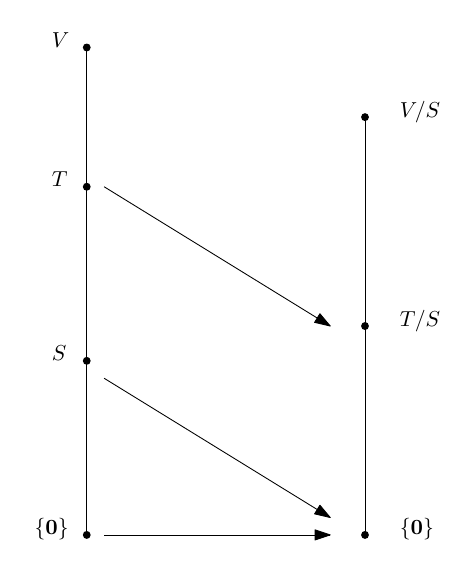
\includegraphics[width=0.37\textwidth]{Figures/correspondence_theorem.png} 
	  \caption{Correspondence between $V$ and $V/S$ \cite{miranda2020avancada}.}
	  \label{fig:correspondence-theorem}
\end{figure}

\begin{theorem}[Universal Property of Quotient]\label{thm:universal_quotient}
	Let $V, W$ vector spaces over $\mathbb{F}$ and $T \in \Hom(V, W)$. If $U$ is a subspace of $V$ such that $U \subseteq \ker (T)$, then there exists a unique linear mapping 
	\[
		S : V / U \longrightarrow W
	\]
\end{theorem}

\begin{proof}
	We need to show that $S([v]) = T(v)$ for all $v \in V$.

	Since $U \subseteq \ker(T)$, if $v - v' \in U$, then $T(v - v') = 0$. Thus, 
	\[
		T(v') = T(v), \quad \forall~v \in V, ~v' \in [v]
	\]

	Hence, there exists a unique function 
	\begin{equation*}
		\begin{aligned}
			S : V/U &\longrightarrow W \\
			[v] &\longmapsto T(v)
		\end{aligned}
	\end{equation*}

	Given that 
	\[
		S([v_1] + \lambda[v_2]) = S([v_1 + \lambda v_2]) = T(v_1 + \lambda v_2) = T(v_1) + \lambda T(v_2) = S([v_1]) + \lambda S([v_2])
	\]
	it follows that $S$ is linear. 
\end{proof}

% \begin{theorem}\label{thm:202301090948}
% 	Suppose that $T \in \Hom(V,W)$ and $U \subseteq \ker(T)$. There exists a unique $S \in \Hom(V/U, W)$ satisfying $S([v]) = T(v)$ for all $v \in V$.

% 	The transformation $S$ is called the \textbf{transformation induced by $T$ on $V/U$}.
% \end{theorem}

The `universal' here means that for all objects in the category, there is exactly one map from this object to $\mathfrak{1}$, i.e., the \textbf{terminal object}.

% Note that $\ker (\tilde{T}) = 0_{V/\ker (T)}$. Then $\tilde{T}$ is injective and $\text{range}(\tilde{T}) = \text{range}(T)$. Hence,
% \[
% 	V/\ker (T) \cong \text{range}(T)
% \]
% which is the \textbf{First Theorem of Isomorphism}.

\begin{theorem}[First Theorem of Isomorphism]
	If $U = \ker(T)$, then the linear mapping $S$ given by the \hyperref[thm:universal_quotient]{Universal Property of Quotient} induces an isomorphism between $V/U$ and $\text{range}(T)$.

	% https://q.uiver.app/?q=WzAsMyxbMCwwLCJWIl0sWzAsMiwiVi9cXGtlcihUKSJdLFsyLDAsIlQoVikiXSxbMCwyLCJUIl0sWzAsMSwiXFx2YXJwaGkiLDJdLFsxLDIsIlxcY29uZyIsMix7InN0eWxlIjp7ImJvZHkiOnsibmFtZSI6ImRhc2hlZCJ9fX1dXQ==
\[\begin{tikzcd}
	V && {T(V)} \\
	\\
	{V/\ker(T)}
	\arrow["T", from=1-1, to=1-3]
	\arrow["\varphi"', from=1-1, to=3-1]
	\arrow["\cong"', dashed, from=3-1, to=1-3]
\end{tikzcd}\]
\end{theorem}

\begin{proof}
	Consider the linear mapping $R : V/U \longrightarrow \text{range}(T)$ given by $R([v]) = S([v]) = T(v)$ for all $v \in V$. Then $R$ is surjective by definition. 

	On the other hand, 
	\[
		R([v]) = 0 \iff T(v) = 0 \iff v \in U \iff [v] = 0
	\]
	i.e. $R$ is injective.
\end{proof}

It will be necessary to have some language to talk about universal properties. To do that, we introduce the following definition.

\begin{definition}[Universal Pair]
	Consider two `functional' properties $P_1$ and $P_2$, i.e., properties that a function may satisfy. Given two sets $X$ and $U$ and a function $\varphi : X \longrightarrow U$, we say that the pair $(\varphi, U)$ is \textbf{universal} over $X$ w.r.t. $P_1$ and $P_2$ if, for all functions $\psi : X \longrightarrow A$ satisfying $P_1$, there exists a unique function $\tilde{\psi} : U \longrightarrow A$ satisfying $P_2$ such that 
	\[
		\tilde{\psi} \circ \varphi = \psi
	\]

	We say that $\tilde{\psi}$ is the function \textbf{induced} by $\psi$ on $U$ w.r.t. $P_2$ and represent its existence by the following commutative diagram 
	% https://q.uiver.app/?q=WzAsMyxbMCwwLCJYIl0sWzIsMCwiQSJdLFswLDIsIlUiXSxbMCwyLCJcXHZhcnBoaSIsMl0sWzAsMSwiXFxwc2kiXSxbMiwxLCJcXHRpbGRle1xccHNpfSIsMix7InN0eWxlIjp7ImJvZHkiOnsibmFtZSI6ImRhc2hlZCJ9fX1dXQ==
	\[\begin{tikzcd}
		X && A \\
		\\
		U
		\arrow["\varphi"', from=1-1, to=3-1]
		\arrow["\psi", from=1-1, to=1-3]
		\arrow["{\tilde{\psi}}"', dashed, from=3-1, to=1-3]
	\end{tikzcd}\]
\end{definition}

The immediate question is: are universal pairs unique? 

\begin{theorem}[Cancellation Law]
	Suppose that $(\varphi, U)$ is universal over $X$ w.r.t. $P_1$ and $P_2$ and $\psi_1, \psi_2 : U \longrightarrow A$ satisfy $P_2$. If $\psi_1 \circ \varphi$ satisfies $P_1$ and coincide with $\psi_2 \circ \varphi$, then $\psi_1 = \psi_2$.
\end{theorem}

\begin{proof}
	Let $\psi := \psi_1 \circ \varphi$ satisfying $P_1$ and consider the following diagram 
	% https://q.uiver.app/?q=WzAsNCxbMiwwLCJYIl0sWzQsMCwiVSJdLFswLDAsIlUiXSxbMiwyLCJBIl0sWzAsMSwiXFx2YXJwaGkiXSxbMCwyLCJcXHZhcnBoaSIsMl0sWzAsMywiXFxwc2kiXSxbMiwzLCJcXHBzaV8xIiwyXSxbMSwzLCJcXHBzaV8yIl1d
	\[\begin{tikzcd}
		U && X && U \\
		\\
		&& A
		\arrow["\varphi", from=1-3, to=1-5]
		\arrow["\varphi"', from=1-3, to=1-1]
		\arrow["\psi", from=1-3, to=3-3]
		\arrow["{\psi_1}"', from=1-1, to=3-3]
		\arrow["{\psi_2}", from=1-5, to=3-3]
	\end{tikzcd}\]

	The hypothesis $\psi_2 \circ \varphi = \psi_1 \circ \varphi = \psi$ and the universality of $(\varphi, U)$, (i.e. $\tilde{\psi}$ is unique) imply $\psi_1 = \psi_2$.
\end{proof}

\begin{definition}[Compatible with compositions]
	We say that a property $P$ is \textbf{compatible with compositions} if $f \circ g$ satisfies $P$ whenever $f$ and $g$ are functions satisfying $P$. 
\end{definition}

\begin{lemma}\label{lm:202301091107}
	Suppose that
	\begin{enumerate}
		\item The pairs $(\varphi, U)$ and $(\psi, V)$ are universal over $X$ w.r.t. $P_1$ and $P_2$;
		\item The functions $\varphi$ and $\psi$ satisfy $P_1$;
		\item The identity functions $\text{Id}_U$ and $\text{Id}_V$ satisfy $P_2$;
		\item The property $P_2$ is compatible with compositions.
	\end{enumerate}

	Then there exists a unique function $f : U \longrightarrow V$ satisfying $P_2$ such that $\psi = f \circ \varphi$. More than that, $f$ is bijective.
\end{lemma}

\begin{proof}
	Using the universal properties and the hypothesis that $\varphi$ and $\psi$ satisfy $P_1$, we know that there exist unique $\tilde{\psi} : U \longrightarrow V$ and $\tilde{\varphi} : V \longrightarrow U$ satisfying $P_2$ such that 
	\[
		\tilde{\psi} \circ \varphi = \psi \quad \text{ and } \quad \tilde{\varphi} \circ \psi = \varphi
	\]

	Thus, 
	\[
		(\tilde{\varphi} \circ \tilde{\psi}) \circ \varphi = \tilde{\varphi} \circ ( \tilde{\psi} \circ \varphi ) = \tilde{\varphi} \circ \psi = \varphi = \text{Id}_U \circ \varphi
	\]
	and, by the cancellation law, $\tilde{\varphi} \circ \tilde{\psi} = \text{Id}_U$.

	Analogously,
	\[
		(\tilde{\psi} \circ \tilde{\varphi}) \circ \psi = \tilde{\psi} \circ ( \tilde{\varphi} \circ \psi ) = \tilde{\psi} \circ \varphi = \psi = \text{Id}_V \circ \psi
	\]
	shows that $\tilde{\psi} \circ \tilde{\varphi} = \text{Id}_V$.

	Taking $f = \tilde{\psi}$, we finish the proof.

	\[\begin{tikzcd}
		X && V \\
		\\
		U
		\arrow["\varphi"', from=1-1, to=3-1]
		\arrow["\psi", from=1-1, to=1-3]
		\arrow["{\tilde{\psi}}", dashed, from=3-1, to=1-3]
		\arrow["{\tilde{\varphi}}", dashed, from=1-3, to=3-1, yshift=-1.5ex]
	\end{tikzcd}\]
\end{proof}

To end this section, we introduce some usual terminology.

\begin{definition}[Codimension]
	Let $W$ be a subspace of $V$. Then the \textbf{codimension} of $W$ in $V$ is
	\[
		\text{codim}_V W = \dim V/W
	\]
\end{definition}

\begin{definition}[Cokernel and Coimage]
	Let $T : V \longrightarrow W$ be a linear transformation. Then the \textbf{cokernel} of $T$ is the quotient space
	\[
		\text{coker} (T) = W / \text{range}(T)
	\] 

	And the \textbf{coimage} of $T$ is defined as
	\[
		\text{coim} (T) = V / \text{Ker}(T)
	\]
\end{definition}

\begin{theorem}
	Suppose $\dim V = n$ and $W$ is a subspace of $V$ with $\dim W = k$. Then 
	\[
		\dim V/W = \text{codim}_V W = n-k
	\]

	I.e., 
	\[
		\dim(V) = \dim(W) + \dim(V/W)
	\]
\end{theorem}

\begin{proof}
	Follows from the theorem \ref{thm:202301090933} and the rank-nullity theorem.
\end{proof}

\begin{corollary}
	Let $V$ be a finite-dimensional vector space $T : V \longrightarrow V$ a linear transformation. Then 
	\[
		\dim (\ker (T)) = \dim (\text{coker} (T))
	\]
\end{corollary}

\section{Tensor Product of Vector Spaces}

The idea here is to `linearize' the tensor product. We will see the tensor product as a universal property, which relates multilinear functions with linear functions. 

\begin{definition}[Tensor Product]
	Consider the functional properties $P_1 =$ `be $k$-linear' and $P_2 =$ `be linear'. Given a family $V_1, \ldots, V_k$ of vector spaces and $\varphi \in \Hom^k(V_1, \ldots, V_k, V)$, a pair $(\varphi, V)$ is a \textbf{tensor product} of this family if it is universal over $X = V_1 \times \cdots \times V_k$ w.r.t. $P_1$ and $P_2$.
\end{definition}

Put another way, $(\varphi, V)$ is a tensor product for $V_1, \ldots, V_k$ if for all $\psi \in \Hom^k(V_1, \ldots, V_k, W)$ ($W$ is a vector space), there exists a unique $\tilde{\psi} \in \Hom(V, W)$ such that $\tilde{\psi} \circ \varphi = \psi$:
% https://q.uiver.app/?q=WzAsMyxbMCwwLCJWXzEgXFx0aW1lcyBcXGNkb3RzIFxcdGltZXMgVl9rIl0sWzAsMiwiViJdLFsyLDAsIlciXSxbMCwxLCJcXHZhcnBoaSIsMl0sWzAsMiwiXFxwc2kiXSxbMSwyLCJcXHRpbGRle1xccHNpfSIsMl1d
\[\begin{tikzcd}
	{V_1 \times \cdots \times V_k} && W \\
	\\
	V
	\arrow["\varphi"', from=1-1, to=3-1]
	\arrow["\psi", from=1-1, to=1-3]
	\arrow["{\tilde{\psi}}"', dashed, from=3-1, to=1-3]
\end{tikzcd}\]

% Given any bilinear map $\varphi \in \Hom(U \times V, T)$, there exists a unique linear mapping $f : U \otimes V \longrightarrow T$ such that the following diagram commutes.
% % https://q.uiver.app/?q=WzAsMyxbMCwwLCJVIFxcdGltZXMgViJdLFsyLDAsIlQiXSxbMCwyLCJVIFxcb3RpbWVzIFYiXSxbMCwxLCJcXHZhcnBoaSJdLFswLDIsIlxcb3RpbWVzIiwyXSxbMiwxLCJcXGV4aXN0cyEgZiIsMix7InN0eWxlIjp7ImJvZHkiOnsibmFtZSI6ImRhc2hlZCJ9fX1dXQ==
% \[\begin{tikzcd}
% 	{U \times V} && T \\
% 	\\
% 	{U \otimes V}
% 	\arrow["\varphi", from=1-1, to=1-3]
% 	\arrow["\otimes"', from=1-1, to=3-1]
% 	\arrow["{\exists! ~f}"', dashed, from=3-1, to=1-3]
% \end{tikzcd}\]

% Put another way, we have the isomorphism
% \begin{equation*}
% 	\begin{aligned}
% 		\Hom(U \otimes V, T) &\longrightarrow \Hom(U \times V, T) \\
% 		f &\longmapsto f \circ \otimes
% 	\end{aligned}
% \end{equation*}
% In the language of categories, this isomorphism is a universal property.

\begin{theorem}[Existence of tensor product]\label{thm:existence_tensor}
	For all families of vector spaces $V_1, \ldots, V_k$, there exists a tensor product. Moreover, if $(\varphi, V)$ is a tensor product for $V_1, \ldots, V_k$, and $\alpha_j$ is a basis for $V_j$, for all $1 \leq j \leq k$, then $\varphi(\alpha_1 \times \cdots \times \alpha_k)$ is a basis for $V$.
\end{theorem}

\begin{proof}
	Notice that the conditions of the Lemma \ref{lm:202301091107} are satisfied. Thus, it is sufficient to prove the second claim of the theorem for a specific tensor product. We start the proof by constructing a tensor product for which we can also verify the second claim. The fact that a multilinear function is completely determined by its action on a cartesian product of bases will appear thoroughly. 

	Let $\alpha = \alpha_1 \times \cdots \alpha_k$ such that $\dim(V) = \# \alpha$,  $\iota : \alpha \longrightarrow V$ such that $\iota(\alpha)$ is a basis of $V$, and $\varphi \in \Hom^k(V_1, \ldots, V_k, V)$ be the unique function satisfying $\varphi|_\alpha = \iota$. 

	Now it will be sufficient to show that $(\varphi, V)$ is a tensor product for $V_1, \ldots, V_k$, since the claim that $\varphi(\alpha)$ is a basis for $V$ is immediate from the definitions of $V$ and $\varphi$. 

	Let us show that $(\varphi, V)$ satisfies the required universal property.
	
	Given $\psi \in \Hom^k(V_1, \ldots, V_k, W)$, and since $\iota(\alpha)$ is a basis for $V$, there exists a unique $\tilde{\psi} \in \Hom(V, W)$ such that 
	\[
		\tilde{\psi}(\iota(v)) = \psi(v), \quad \forall~v \in \alpha
	\]

	In particular, since $\varphi$ and $\psi$ are $k$-linear, it follows that $\tilde{\psi} \circ \varphi = \psi$. More than that, if $\xi \in \Hom(V, W)$ satisfies $\xi \circ \varphi = \psi$, then for all $v \in \alpha$, 
	\[
		\xi(\iota(v)) = \xi(\varphi(v)) = \psi(v) 
	\]
	and, therefore, $\xi = \tilde{\psi}$. 
\end{proof}

In a certain sense, the tensor product is the `price' of linearization. An alternative proof of the Theorem \ref{thm:existence_tensor} is given at the \hyperref[thm:existence_tensor_alt]{end of this section}.

\begin{theorem}\label{thm:202301121102}
	If $(\varphi, V)$ is a tensor product for $V_1, \ldots, V_k$, then for all vector space $W$, there exists an isomorphism 
	\begin{equation*}
		\begin{aligned}
			\Gamma : \Hom^k (V_1, \ldots, V_k, W) &\longrightarrow \Hom(V,W) \\
			\psi &\longmapsto \tilde{\psi}
		\end{aligned}
	\end{equation*}
\end{theorem}

\begin{proof}
	The universality of $\varphi$ defines $\Gamma$ uniquely. To show that $\Gamma$ is surjective, given $\tau \in \Hom(V,W)$, take $\psi = \tau \circ \varphi$, which is $k$-linear and, therefore, $\tau = \tilde{\psi} = \Gamma(\psi)$. 

	To prove injectivity, suppose that $\psi, \xi \in \Hom^k (V_1, \ldots, V_k, W)$ satisfy $\tilde{\psi} = \tilde{\xi}$. Then \[ \psi = \tilde{\psi} \circ \varphi = \tilde{\xi} \circ \varphi = \xi \]

	Let us show that $\Gamma$ is linear. Given a scalar $\lambda$, 
	\[
		\Gamma(\psi) + \lambda \Gamma(\xi) = \tilde{\psi} + \lambda \tilde{\xi}
	\]

	On the other hand, $\Gamma(\psi + \lambda \xi)$ is the only element of $\Hom (V, W)$ such that $\Gamma(\psi + \lambda \xi) \circ \varphi = \psi + \lambda \xi$. Thus, we need to verify that 
	\[
		(\tilde{\psi} + \lambda \tilde{\xi}) \circ \varphi = \psi + \lambda \xi
	\]

	In fact, given $v_j \in V_j$, for all $1 \leq j \leq k$, we have 
	\begin{equation*}
		\begin{aligned}
			(\tilde{\psi} + \lambda \tilde{\xi})(\varphi(v_1, \ldots, v_k)) &= \tilde{\psi}(\varphi(v_1, \ldots, v_k)) + \lambda \tilde{\xi}(\varphi(v_1, \ldots, v_k)) \\
			&= \psi (v_1, \ldots, v_k) + \lambda \xi (v_1, \ldots, v_k) \\
			&= (\psi + \lambda \xi) (v_1, \ldots, v_k)
		\end{aligned}
	\end{equation*}

	Hence, $\Gamma$ is an isomorphism.
\end{proof}

The isomorphism in the previous theorem is a canonical isomorphism.

For the sake of simplicity, we introduce the following notation.

\begin{definition}[Tensor Notation]
	We will denote by $V_1 \otimes \cdots \otimes V_k$ the vector space of the universal pair of a tensor product for $V_1, \ldots, V_k$ and the corresponding $k$-linear function of the pair by $\otimes$. 

	Given $v_j \in V_j$, for all $1 \leq j \leq k$, we will use the notation 
	\[
		v_1 \otimes \cdots \otimes v_k = \otimes(v_1, \ldots, v_k)
	\]

	When it is necessary to specify the field, we'll use the symbol $\otimes_{\mathbb{F}}$.
\end{definition}

Notice that the $k$-linearity of $\otimes$ can be rewritten as 
\begin{equation*}
	\begin{aligned}
		v_1 \otimes \cdots \otimes v_{j-1} &\otimes (v_j + \lambda v_j') \otimes v_{j+1} \otimes \cdots \otimes v_k = \\ 
		&(v_1 \otimes \cdots \otimes v_k) + \lambda (v_1 \otimes \cdots \otimes v_{j-1} \otimes v_j' \otimes v_{j+1} \otimes \cdots \otimes v_k)
	\end{aligned}
\end{equation*}
for any $v_j, v_j' \in V_j$, $1 \leq j \leq k$, and $\lambda \in \mathbb{F}$.

\begin{theorem}[Associativity of the Tensor Product]
	Given $1 \leq l < k$, there exists a unique isomorphism of vector spaces 
	\[
		\Gamma : V_1 \otimes \cdots \otimes V_k \longrightarrow (V_1 \otimes \cdots \otimes V_l) \otimes (V_{l+1} \otimes \cdots \otimes V_k)
	\]
	satisfying $\Gamma(v_1 \otimes \cdots \otimes v_k) = (v_1 \otimes \cdots \otimes v_l) \otimes (v_{l+1} \otimes \cdots \otimes v_k)$ for any $v_j \in V_j$ and $1 \leq j \leq k$.
\end{theorem}

\begin{proof}
	Let $V = V_1 \otimes \cdots \otimes V_k$ and $W = (V_1 \otimes \cdots \otimes V_l) \otimes (V_{l+1} \otimes \cdots \otimes V_k)$.

	Consider the function $\psi : V_1 \times \cdots \times V_k \longrightarrow W$ given by 
	\[
		(v_1, \ldots, v_k) \longmapsto (v_1 \otimes \cdots \otimes v_l) \otimes (v_{l+1} \otimes \cdots \otimes v_k)
	\]
	for any $v_j \in V_j$ and $1 \leq j \leq k$, which $k$-linear.

	By the universal property of $V$, there exists a unique $\Gamma \in \Hom(V, W)$ satisfying 
	\[
		\Gamma (v_1, \ldots, v_k) = (v_1 \otimes \cdots \otimes v_l) \otimes (v_{l+1} \otimes \cdots \otimes v_k)
	\]
	for any $v_j \in V_j$ and $1 \leq j \leq k$.

	% https://q.uiver.app/?q=WzAsMyxbMCwwLCJWXzEgXFx0aW1lcyBcXGNkb3RzIFxcdGltZXMgVl9rIl0sWzAsMiwiViJdLFsyLDAsIlciXSxbMCwxLCJcXG90aW1lcyIsMl0sWzAsMiwiXFxwc2kiXSxbMSwyLCJcXEdhbW1hIiwyXV0=
	\[\begin{tikzcd}
		{V_1 \times \cdots \times V_k} && W \\
		\\
		V
		\arrow["\otimes"', from=1-1, to=3-1]
		\arrow["\psi", from=1-1, to=1-3]
		\arrow["\Gamma"', from=3-1, to=1-3]
	\end{tikzcd}\]

	By the second part of the Theorem \ref{thm:existence_tensor}, $\Gamma$ takes basis into basis and, therefore, is an isomorphism.
\end{proof}

How does the tensor product of subspaces relate to the tensor product of the original spaces? 

\begin{theorem}\label{thm:202301091423}
	If $V_j'$ is a subspace of $V_j$, for all $1 \leq j \leq k$, there exists a unique linear transformation 
	\begin{equation*}
		\begin{aligned}
			\Gamma : V_1' \otimes \cdots \otimes V_k' & \longrightarrow V_1 \otimes \cdots \otimes V_k \\
			v_1 \otimes \cdots \otimes v_k &\longmapsto v_1 \otimes \cdots \otimes v_k
		\end{aligned}
	\end{equation*}
	for any $v_j \in V_j'$ and $1 \leq j \leq k$. Moreover, $\Gamma$ is injective.
\end{theorem}

Using identity functions, we may interpret $V_1' \otimes \cdots \otimes V_k'$ as a subspace of $V_1 \otimes \cdots \otimes V_k$.

As a consequence of the theorem \ref{thm:202301091423}, $v_1 \otimes \cdots \otimes v_k = 0$ iff. $v_j = 0$ for some $1 \leq j \leq k$.

\begin{definition}[Pure Tensors]
	Vectors of the form $v_1 \otimes \cdots \otimes v_k$ are called \textbf{homogeneous vectors} or \textbf{pure tensors}.
\end{definition}

By the second part of the Theorem \ref{thm:existence_tensor}, the homogeneous vectors span $V_1 \otimes \cdots \otimes V_k$. More than that, since a scalar multiple of a pure tensor is again a pure tensor, every vector of $V_1 \otimes \cdots \otimes V_k$ can be represented as a sum of homogeneous vectors:
\begin{equation}\label{eq:202301091429}
	v = \sum_{i=1}^m v_{i,1} \otimes \cdots \otimes v_{i,k}
\end{equation}
for some choice of $m \in \mathbb{Z}_{\geq 0}$ and $v_{i,j} \in V_j \setminus \{ 0 \}$.

\begin{definition}[Tensor Rank]
	The minimal amount of parts in \eqref{eq:202301091429} is called the \textbf{rank} of $v$ and is denoted by $\text{rank}(v)$.
\end{definition}

The rank of the null vector is zero and the rank of nonzero homogeneous vectors is one.

\begin{example}[Impure tensor]
	Let $V = \mathbb{F}^2$ and let us show that the rank of the following vector of $V^{\otimes 3}$ is two: 
	\[
		v = e_1 \otimes e_1 \otimes e_1 + e_2 \otimes e_1 \otimes e_2
	\]

	Notice that the parts on the definition of $v$ form a linearly independent family on $V^{\otimes 3}$ and, therefore, $0 < \text{rank}(v) \leq 2$. 

	If $\text{rank}(v) = 1$, there must exist a family $v_1, v_2, v_3$ such that $v = v_1 \otimes v_2 \otimes v_3$. Each $v_i$ would be of the form 
	\[
		v_i = a_{i,1} e_1 + e_{i,2} e_2
	\]

	Using the $3$-linearity of $\otimes$, we can write $v_1 \otimes v_2 \otimes v_3$ in the basis $(e_i \otimes e_j \otimes e_k)$, where $1 \leq i,j,k \leq 2$. This gives us a nonlinear system without solution. 

	Hence, $\text{rank}(v) = 2$.
\end{example}

% The case of two factors will be proven important

\begin{lemma}\label{lm:202301100826}
	If $u = v_1 \otimes w_1 + \cdots + v_m \otimes w_m \in V \otimes W$ has rank $m$, then $(v_i)_i$ and $(w_i)_i$ are linearly independent. Hence, \[ \text{rank}(u) \leq \min \{ \dim(V), \dim(W) \}, \quad \forall~u \in V \otimes W \]
\end{lemma}

\begin{proof}
	Suppose that 
	\[
		w_m = a_1 w_1 + \cdots + a_{m-1} w_{m-1}, \quad a_j \in \mathbb{F}, ~1 \leq j < m
	\]

	It follows that 
	\[
		v_m \otimes w_m = \sum_{j=1}^{m-1} (a_j v_m) \otimes w_j
	\]
	and, therefore, 
	\[
		u = \sum_{j=1}^{m-1} (v_j + a_j v_m) \otimes w_j
	\]
	contradicting the fact that $\text{rank}(u) = m$.
\end{proof}

\begin{lemma}\label{lm:202301100835}
	Let $\alpha = v_1, \ldots, v_m$ and $\alpha' = v_1', \ldots, v_p'$ be families on $V$, and $\beta = w_1, \ldots, w_m$ and $\beta' = w_1', \ldots, w_p'$ be families on $W$ such that 
	\[
		\sum_{j=1}^{m} v_j \otimes w_j = \sum_{i=1}^{p} v_i' \otimes w_i'
	\]
	
	If $\alpha, \alpha'$ and $\beta'$ are linearly independent, then $[\beta] \subseteq [\beta']$. In particular, if $p = 0$, then $w_j = 0$ for all $1 \leq j \leq m$.
\end{lemma}

\begin{proof}
	We proceed by induction on $p$. For $p = 0$, we use induction on $m \geq 1$, which starts when $m = 1$ since $v_1 \otimes \cdots \otimes v_k = 0$ iff. $v_j = 0$ for some $1 \leq j \leq k$ (see Theorem \ref{thm:202301091423}). 

	If $w_1, \ldots, w_m$ were linearly independent, then each part $v_j \otimes w_j$ would be a part of a basis for $V \otimes W$, contradicting $v_1 \otimes w_1 + \cdots + v_m \otimes w_m = 0$. 

	Thus, we can suppose w.l.o.g. that $w_m = a_1 w_1 + \cdots + a_{m-1} w_{m-1}$ and, using the lemma \ref{lm:202301100826}, it follows that 
	\[
		\sum_{j=1}^{m-1} (v_j + a_j v_m) \otimes w_j = 0
	\]

	Notice that $(v_j + a_j v_m)_{1 \leq j < m}$ is linearly independent. Using the induction hypothesis, $w_j = 0$ for $1 \leq j < m$. Then $v_m \otimes w_m = 0$ and, by the case $m = 1$, $w_m = 0$.

	For $p > 0$, if $\alpha \cup \alpha'$ is linearly independent, the case $p = 0$ implies that $w_j = w_i' = 0$, contradicting the fact that $\beta'$ is linearly independent. We can rewrite 
	\[
		\sum_{j=1}^{m} v_j \otimes w_j + \sum_{i=1}^{p} v_i' \otimes (-w_i') = 0
	\]

	Therefore, $\alpha \cup \alpha'$ is linearly dependent. We can suppose, w.l.o.g. that 
	\[
		v_p' = a_1 v_1 + \cdots + a_mv_m + a_1' v_1' + \cdots + a_{p-1}' v_{p-1}'
	\]

	Using calculations similar to the lemma \ref{lm:202301100826}, we obtain 
	\[
		\sum_{j=1}^{m} v_j \otimes (w_j - a_j w_p') = \sum_{i=1}^{p-1} v_i' \otimes (w_i' + a_i' w_p')
	\]

	Since the family $\beta^{''} = (w_i' + a_i' w_p')_{1 \leq i < p}$ is linearly independent, by the induction hypothesis on $p$, we have that $w_j - a_j w_p' \in [\beta^{''}]$ for all $1 \leq j \leq m$. 

	Since $[\beta^{''}] \subseteq [\beta']$, it follows that $w_j \in [\beta']$ for all $1 \leq j \leq m$. 
\end{proof}

\begin{theorem}\label{thm:202301101040}
	If $\alpha = v_1, \ldots, v_m$ is a linearly independent family on $V$ and $\beta = w_1, \ldots, w_m$ is a linearly independent family on $W$, then the rank of $u = v_1 \otimes w_1 + \cdots + v_m \otimes w_m$ is $m$. 
\end{theorem}

\begin{proof}
	Let $p = \text{rank}(u)$. In particular, $m \geq p$. 

	Let $\alpha' = v_1', \ldots, v_p'$ and $\beta' = w_1', \ldots, w_p'$ such that 
	\[
		u = v_1' \otimes w_1' + \cdots + v_p' \otimes w_p'
	\]

	Notice that $\alpha'$ and $\beta'$ are linearly independent by the lemma \ref{lm:202301100826}. Thus, it follows from the lemma \ref{lm:202301100835} that $[\beta] \subseteq [\beta']$. Since $\beta$ is linearly independent, we have that $m \leq p$. 
\end{proof}

\begin{example}
	If $V = W = \mathbb{Q}^2$, $\text{rank}(5 e_1 \otimes e_1  - 3 e_2 \otimes e_2) = 2$. 

	Let us compute the rank of 
	\[
		u = (e_1 + e_2) \otimes (e_1 - e_2) + (e_1 + 2 e_2) \otimes e_2 + (e_1 - e_2) \otimes (e_1 + e_2)
	\]

	Since $(e_1 + e_2) = (e_1 - e_2) + 2 e_2$, 
	\begin{equation*}
		\begin{aligned}
			u &= (e_1 + e_2 + e_1 - e_2) \otimes (e_1 - e_2) + (e_1 + 2 e_2 + 2(e_1 - e_2)) \otimes e_2 \\
			&= (2e_1) \otimes (e_1 - e_2) + (3 e_1) \otimes e_2 = e_1 \otimes (2 (e_1 - e_2) + e_2) \\
			&= e_1 \otimes (2 e_1 + e_2)
		\end{aligned}
	\end{equation*}

	Hence, $\text{rank}(u) = 1$.
\end{example}

The next result shows a `translation' between the language of linear transformations and the language of tensors.

\begin{theorem}\label{thm:translation_lt_tensor}
	There exists a unique linear mapping $\Gamma : V^\ast \otimes W \longrightarrow \Hom (V, W)$ satisfying 
	\[
		\Gamma(f \otimes w)(v) = f(v)w, \quad \forall~ v \in V, ~w \in W, ~f \in V^\ast
	\]

	Furthermore, 
	\begin{enumerate}
		\item $\Gamma$ is injective;
		\item For all $u \in V^\ast \otimes W$, $\text{rank}(\Gamma(u)) = \text{rank}(u)$; 
		\item $T \in \text{range}(\Gamma)$ iff. $\text{rank}(T)$ is finite; 
		\item $\Gamma$ is surjective iff. $\dim(V)$ or $\dim(W)$ is finite. 
	\end{enumerate}
\end{theorem}

\begin{proof}
	Notice that the function $\psi : V^\ast \otimes W \longrightarrow \Hom (V, W)$ given by $\psi(f, w)(v) = f(v)w$ is well defined. In fact, 
	\begin{equation*}
		\begin{aligned}
			\psi (f, w)(v_1 + \lambda v_2) &= f(v_1 + \lambda v_2) w \\
			&= (f(v_1)w) + \lambda(f(v_2)w) \\
			&= \psi(f, w)(v_1) + \lambda \psi (f,w)(v_2)
		\end{aligned}
	\end{equation*}

	It can be easily verified that $\psi$ is bilinear. Thus, the existence of $\Gamma = \tilde{\psi}$ follows from the universal property of $V^\ast \otimes W$. 

	Since $\text{rank}(T) \leq \min \{ \dim(V), \dim(W) \}$, the third item implies the fourth. 

	To show the first item, let $u \in \ker(\Gamma)$ and write
	\begin{equation}\label{eq:202301101035}
		u = \sum_{j=1}^{m} f_j \otimes w_j, \quad \text{ with } (f_j), ~(w_j) \text{ l.i.}
	\end{equation}

	If $m > 0$, since $f_1 \neq 0$, then there exists $v \in V$ such that $f_1(v) \neq 0$ and thus 
	\begin{equation}\label{eq:202301101048}
		0 = \Gamma(u)(v) = \sum_{j=1}^{m} f_j(v) w_j
	\end{equation}
	contradicts the fact that $(w_j)$ is linearly independent. Hence, $m = 0$ and $\Gamma$ is injective. 

	To prove the second item, using an expression like \eqref{eq:202301101035}, let $W' = [ w_1, \ldots, w_m ]$. Using the Theorem \ref{thm:202301101040}, we have that $\dim(W') = \text{rank}(u)$. Thus it suffices to show that $\text{range}(\Gamma(u)) = W'$. 

	Looking at the equation \eqref{eq:202301101048} it is immediate that $\text{range}(\Gamma(u)) \subseteq W'$ and we need to prove that $w_j \in \text{range}(\Gamma(u))$ for all $1 \leq j \leq m$. Since, for all $1 \leq j \leq m$, there exists $v \in V$ such that $f_i(v) = \delta_{i,j}$, for all $1 \leq i \leq m$, we have that $\Gamma(u)(v) = w_j$.

	Now we prove the third item. Let $F = \{ T \in \Hom(V,W) : \text{rank}(T) < \infty \}$. The second item implies that every element in the range has a finite rank, since the tensor rank is always finite, i.e., $\text{range}(\Gamma) \subseteq F$. 

	Reciprocally, if $T \in F$ with $\text{rank}(T) = m$, choose a basis $\{ w_1, \ldots, w_m \}$ for $\text{range}(T)$. Given a basis $\alpha = (v_i)_{i \in I}$ for $V$, we have 
	\[
		T(v_i) = \sum_{j=1}^{m} a_{i,j} w_j, \quad a_{i,j} \in \mathbb{F}
	\]

	For each $1 \leq j \leq m$ let $f_j$ be the only element of $V^\ast$ satisfying $f_j(v_i) = a_{i,j}$ for all $i \in I$. It follows that
	\[
		\Gamma \left( \sum_{j=1}^{m} f_j \otimes w_j \right)(v_i) = \sum_{j=1}^{m} f_j(v_i) \otimes w_j = \sum_{j=1}^{m} a_{i,j} \otimes w_j = T(v_i)
	\]
\end{proof}

This result motivates a simple way to compute the tensor rank using matrices.

Let $\alpha = v_1, \ldots, v_m$ be a basis for $V$ and $\beta = w_1, \ldots, w_m$ be a basis for $W$. And also let $\alpha^\ast = \{ f_1, \ldots, f_n \}$ be the dual basis of $\alpha$ and $\Gamma$ be the function in the Theorem \ref{thm:translation_lt_tensor}. Then 
\[
	\Gamma(f_j \otimes w_i)(v_k) = \delta_{k,j} w_i
\]
and, therefore, 
\[
	[\Gamma(f_j \otimes w_i)]_\beta^\alpha = E_{i,j}
\]

Hence, if $ A = (a_{i,j}) \in M_{m,n}(\mathbb{F})$ and $T \in \Hom(V, W)$ is given by $[T]_\beta^\alpha = A$, then 
\begin{equation}\label{eq:202301101119}
	T = \Gamma \left( \sum_{i=1}^{m} \sum_{j=1}^{n} a_{i,j} ~f_j \otimes w_i \right)
\end{equation}

From this fact, the rank of each element of $V^\ast \otimes W$ coincides with the rank of the corresponding matrix w.r.t. the basis $\alpha^\ast$ and $\beta$.

We also obtain that to compute the rank of a tensor, it suffices to write the tensor in a given basis and row-reduce the matrix of the coordinates. 

How can we interpret the trace in the context of tensors? 

\begin{theorem}[Tensor Trace]
	There exists a unique $\tau \in (V^\ast \otimes V)^\ast$ satisfying 
	\[
		\tau (f \otimes v) = f(v), \quad \forall~f \in V^\ast, ~v \in V
	\]

	Additionally, if $\dim(V) < \infty$ and $\Gamma : V^\ast \otimes V \longrightarrow \End(V)$ as in the Theorem \ref{thm:translation_lt_tensor}, then $\tau(\Gamma^{-1}(T)) = \text{tr}(T)$. 
\end{theorem}

\begin{proof}
	The existence and uniqueness part follows from the universal property of the tensor product. 

	To justify $\tau(\Gamma^{-1}(T)) = \text{tr}(T)$, suppose that $\alpha = \{ v_1, \ldots, v_n \}$ is a basis for $V$ and $\alpha^\ast = \{ f_1, \ldots, f_n \}$ is the dual basis of $\alpha$. 

	Using \eqref{eq:202301101119}, if $[T]_\alpha^\alpha$, then 
	\[
		\Gamma^{-1}(T) = \sum_{i=1}^{n} \sum_{j=1}^{n} a_{i,j} ~f_j \otimes v_i
	\]

	Thus, 
	\[
		\tau(\Gamma^{-1}(T)) = \sum_{i=1}^{n} \sum_{j=1}^{n} a_{i,j} ~\tau(f_j \otimes v_i) = \sum_{i=1}^{n} \sum_{j=1}^{n} a_{i,j} ~f_j(v_i) = \sum_{i=1}^{n} a_{i,i}
	\]
\end{proof}

We finish this section with an alternative proof for the existence of tensor product (Theorem \ref{thm:existence_tensor}). 

\begin{proof}\label{thm:existence_tensor_alt}
	Let $X = V_1 \times \cdots \times V_k$ and $(\alpha, L)$ be a universal pair over $X$ w.r.t. properties $P_1 =$ `is a vector space over $\mathbb{F}$' and $P_2 =$ `is linear', i.e., $\alpha : X \longrightarrow L$ indexes a basis for $L$. 

	Since $\alpha$ is a basis, it is injective and we can identify $X$ with its range on $L$. Thus the element $(v_1, \ldots, v_k)$ will be interpreted as a vector on $L$, where each $v_j \in V_j$, i.e., we're looking to the image of $(v_1, \ldots, v_k)$ by $\alpha$.
	
	Now consider the subspace $K \subseteq L$ spanned by all vectors of the form 
	\begin{equation}\label{eq:202301121556}
		\begin{aligned}
			(v_1, \ldots, v_{j-1}, \lambda v_j, v_{j+1}, \ldots, v_k) &- \lambda (v_1, \ldots, v_k), \quad \text{ and } \\
			(v_1, \ldots, v_{j-1}, v_j + v_j', v_{j+1}, \ldots, v_k) &- (v_1, \ldots, v_k) - (v_1, \ldots, v_{j-1}, v_j', v_{j+1}, \ldots, v_k)
		\end{aligned}
	\end{equation}
	with $v_j, v_j' \in V_j$ and $\lambda \in \mathbb{F}$. Define 
	\[
		V = L/K \quad \text{ and } \quad \varphi = \pi \circ \alpha
	\]
	where $\pi : L \longrightarrow L/K$ is the canonical projection. 

	Let us show that $(\varphi, V)$ is a tensor product for $V_1, \ldots, V_k$. By the equation \eqref{eq:202301121556}, we have that 
	\begin{equation*}
		\begin{aligned}
			\varphi (v_1, \ldots, v_{j-1}, \lambda v_j, v_{j+1}, \ldots, v_k) &= \lambda \varphi (v_1, \ldots, v_k), \quad \text{ and } \\
			\varphi (v_1, \ldots, v_{j-1}, v_j + v_j', v_{j+1}, \ldots, v_k) &= \varphi (v_1, \ldots, v_k) + \varphi (v_1, \ldots, v_{j-1}, v_j', v_{j+1}, \ldots, v_k)
		\end{aligned}
	\end{equation*}
	i.e., $\varphi$ is $k$-linear. Now we need to show that $(\varphi, V)$ satisfies the desired universal property. 

	Given $\psi \in \Hom^k(V_1, \ldots, V_k, W)$, since $\alpha$ is a basis for $L$, there exists a unique $T \in \Hom(L, W)$ such that 
	\[
		T(v_1, \ldots, v_k) = \psi(v_1, \ldots, v_k), \quad \forall ~v_j \in V_j, ~1 \leq j \leq k
	\]

	Since $\psi$ is $k$-linear, the generating vectors of $K$, described in \eqref{eq:202301121556}, are in the nullspace of $T$, i.e., $K \subseteq \ker(T)$. By the \hyperref[thm:universal_quotient]{Universal Property of the Quotient}, there exists a unique $\tilde{\psi} \in \Hom(V,W)$ satisfying 
	\[
		\tilde{\psi} (\pi(u)) = T(u), \quad \forall~u \in L
	\]

	In particular, $\tilde{\psi} \circ \varphi = \psi$.
	
	What remains to be proved now is the uniqueness of $\tilde{\psi}$, i.e., that if $\xi \in \Hom(V,W)$ satisfies $\xi \circ \varphi = \psi$, then $\xi = \tilde{\psi}$. Notice that the properties 
	\[
		\tilde{\psi} \circ \varphi = \psi \quad \text{ and } \quad \xi \circ \varphi = \psi
	\]
	imply that $\tilde{\psi}$ and $\xi$ coincide in $\text{range}(\varphi)$. However, $\text{range}(\varphi)$ spans $V$, since $\alpha$ spans $L$ and $\pi$ is surjective. Hence, $\xi = \tilde{\psi}$, completing the proof that $(\varphi, V)$ is a tensor product. 
\end{proof}

\section{Tensor Product of Linear Mappings}

In this section we study the tensor product of linear transformations, which can be interpreted as linear transformation. 

Given $T_j \in \Hom (V_j, W_j)$, for $1 \leq j \leq k$, consider the $k$-linear function 
\begin{equation*}
	\begin{aligned}
		\psi : V_1 \times \cdots \times V_k &\longrightarrow W_1 \otimes \cdots \otimes W_k \\
		(v_1, \ldots, v_k) &\longmapsto T_1(v_1) \otimes \cdots \otimes T_k(v_k)
	\end{aligned}
\end{equation*}

Notice that this function is a generalization of the evaluation function. Now consider the induced linear mapping 
\begin{equation*}
	\begin{aligned}
		\tilde{\psi} : V_1 \otimes \cdots \otimes V_k &\longrightarrow W_1 \otimes \cdots \otimes W_k \\
		v_1 \otimes \cdots \otimes v_k &\longmapsto T_1(v_1) \otimes \cdots \otimes T_k(v_k)
	\end{aligned}
\end{equation*}

Thus, we can define a function 
\begin{equation*}
	\begin{aligned}
		\varphi : \Hom (V_1, W_1) \times \cdots \times \Hom (V_k, W_k) &\longrightarrow \Hom (V_1 \otimes \cdots \otimes V_k, ~W_1 \otimes \cdots \otimes W_k) \\
		(T_1, \ldots, T_k)(v_1 \otimes \cdots \otimes v_k) &\longmapsto T_1(v_1) \otimes \cdots \otimes T_k(v_k)
	\end{aligned}
\end{equation*}

Note that $\varphi$ is $k$-linear and we have the induced linear transformation
\begin{equation*}
	\begin{aligned}
		\tilde{\varphi} : \Hom (V_1, W_1) \otimes \cdots \otimes \Hom (V_k, W_k) &\longrightarrow \Hom (V_1 \otimes \cdots \otimes V_k, ~W_1 \otimes \cdots \otimes W_k) \\
		T_1 \otimes \cdots \otimes T_k &\longmapsto \varphi (T_1, \ldots, T_k)
	\end{aligned}
\end{equation*}

\begin{definition}[Tensor Product of Linear Transformations]
	The linear transformation \[ \tilde{\psi} = \varphi (T_1, \ldots, T_k) \] will be denoted by $T_1 \otimes \cdots \otimes T_k$ and will be called the \textbf{tensor product} of the family $T_1, \ldots, T_k$.
\end{definition}

\begin{lemma}\label{lm:202301111112}
	The following are true.
	\begin{enumerate}
		\item $\text{range}(T_1 \otimes \cdots \otimes T_k) = \text{range}(T_1) \otimes \cdots \otimes \text{range}(T_k)$.
		\item Let $N_j = V_j \otimes \cdots \otimes V_{j-1} \otimes \ker(T_j) \otimes V_{j+1} \otimes \cdots \otimes V_k$, for $1 \leq j \leq k$. Then $\ker(T_1 \otimes \cdots \otimes T_k) = N_1 + \cdots + N_k$. In particular, $T_1 \otimes \cdots \otimes T_k$ is injective if $T_j$ is injective for all $1 \leq j \leq k$.
	\end{enumerate}
\end{lemma}

\begin{proof}
	$(1.)$ \textbf{Exercise.}

	$(2.)$ The second claim is immediate from the first since $N_j = \{ 0 \}$.
	
	The fact that $N_j \subseteq \ker (T_1 \otimes \cdots \otimes T_k)$ is evident e, and therefore, if $N := N_1 + \cdots + N_k$, we have $N \subseteq \ker (T_1 \otimes \cdots \otimes T_k)$. 
	
	Let $V + V_1 \otimes \cdots \otimes V_k$ and $W = \text{range}(T_1) \otimes \cdots \otimes \text{range}(T_k) = \text{range}(T_1 \otimes \cdots \otimes T_k)$. Consider the canonical projection $\pi : V \longrightarrow V/N$. We'll show that there exists $S \in \Hom (W, V/N)$ such that 
	\begin{equation}\label{eq:202301111124}
		S \circ (T_1 \otimes \cdots \otimes T_k) = \pi
	\end{equation}

	If this is the case,
	\[ 
		\ker(T_1 \otimes \cdots \otimes T_k) \subseteq \ker(S \circ (T_1 \otimes \cdots \otimes T_k)) \overset{\eqref{eq:202301111124}}{=} N
	\]
	and the lemma follows. 

	We need to show how to define $S$ satisfying \eqref{eq:202301111124}. For each $1 \leq j \leq k$, let $\sigma_j$ be a right inverse for $T_j$, i.e., $\sigma_j : \text{range}(T_j) \longrightarrow V_j$ satisfies 
	\[
		T_j(\sigma_j(w)) = w, \quad \forall~w \in \text{range}(T_j)
	\]

	Since $T_j(\sigma_j(T_j(v)) - v) = T_j(\sigma_j (T_j(v))) - T_j(v) = 0$, this implies that 
	\begin{equation}\label{eq:202301111130}
		\sigma_j(T_j(v)) - v \in \ker(T_j), \quad \forall ~v \in V_j
	\end{equation}

	Define 
	\begin{equation*}
		\begin{aligned}
			\text{range}(T_1) \times \cdots \times \text{range}(T_k) &\longrightarrow V/N \\
			(w_1, \ldots, w_k) &\longmapsto \pi(\sigma_1(w_1) \otimes \cdots \otimes \sigma_k (w_k))
		\end{aligned}
	\end{equation*}

	We now show that $\sigma$ is $k$-linear and that $S := \tilde{\sigma}$ satisfies \eqref{eq:202301111124}.

	Given $v_j \in V_j$, \eqref{eq:202301111130} implies that there exists $v_j \in \ker(T_j)$ such that $\sigma_j(T_j(v_j)) = v_j + v_j'$. Then 
	\begin{equation*}
		\begin{aligned}
		\tilde{\sigma}((T_1 \otimes \cdots \otimes T_k)(v_1 \otimes \cdots \otimes v_k)) &= \tilde{\sigma}(T_1(v_1) \otimes \cdots \otimes T_k(v_k)) \\
		&= \sigma(T_1(v_1), \ldots, T_k(v_k)) \\
		&= \pi(\sigma_1(T_1(v_1)) \otimes \cdots \otimes \sigma_k(T_k(v_k))) \\
		&= \pi((v_1 + v_1') \otimes \cdots \otimes (v_k + v_k')) \\
		&= \pi(v_1 \otimes \cdots \otimes v_k) + \pi (v_1' \otimes \cdots \otimes v_k')
		\end{aligned}
	\end{equation*}
	where $v_1' \otimes \cdots \otimes v_k'$ is a sum of elements on $N$, proving that $\tilde{\sigma}$ satisfies \eqref{eq:202301111124}.

	Recall that for every surjective linear transformation, there exists a right inverse which is also linear. Using this fact, we prove that $\sigma$ is $k$-linear.
\end{proof}

\begin{theorem}\label{thm:202301110932}
	The linear mapping $\tilde{\varphi}$ is injective. If $V_j$ and $W_j$ are finite-dimensional for all $1 \leq j \leq k$, then $\tilde{\varphi}$ is an isomorphism.
\end{theorem}

\begin{proof}
	The second claim follows form the first one, since domain and codomain have the same finite dimension. 

	We proceed by induction on $k \geq 2$. For $k = 2$, let $\Gamma \in \ker(\tilde{\varphi})$ and choose an expression for $\Gamma$ of the form 
	\[
		\Gamma = \sum_{j=1}^{m} T_j \otimes S_j
	\]
	where $T_j \in \Hom (V_1, W_1)$ and $S_j \in \Hom (V_2, W_2)$ such that $T_1, \ldots, T_m$ and $S_1, \ldots, S_m$ are linearly independent families. In particular,
	\begin{equation}\label{eq:202301110940}
		\tilde{\varphi}(\Gamma)(v, v') = \sum_{j=1}^{m} T_j(v) \otimes S_j(v') = 0, \quad \forall ~v \in V_1, ~v' \in V_2
	\end{equation}

	Our goal is to show that $m = 0$. If $m \neq 0$, then $T_1 \neq 0$ and we can choose $v \in V_1$ such that $T_1(v) \neq 0$. 

	Let $r$ be the dimension of the subspace of $W_1$ spanned by $T_1(v), \ldots, T_m(v)$ and suppose, w.l.o.g., that $T_1(v), \ldots, T_r(v)$ is linearly independent. 

	Thus, for each $r < l \leq m$, there exist scalars $a_{i,l}$, where $1 \leq i \leq r$, such that 
	\[
		T_l(v) = \sum_{i=1}^{r} a_{i,l} T_i(v)
	\]

	Applying these expressions in \eqref{eq:202301110940}, 
	\[
		\sum_{j=1}^{r} T_j(v) \otimes \left( S_j(v') + \sum_{l=r+1}^{m} a_{j,l} S_l(v') \right) = 0
	\]

	Since $T_1(v), \ldots, T_r(v)$ is linearly independent, it follows from the Lemma \ref{lm:202301100835} that 
	\[
		S_j + \sum_{l=r+1}^{m} a_{j,l} S_l = 0, \quad \forall~1 \leq j \leq r
	\]
	contradicting the fact that $S_1, \ldots, S_m$ is linearly independent. Hence, $m = 0$ and $\Gamma = 0$, completing the proof for $k = 2$.

	Suppose that $k > 2$ and define 
	\[
		V = V_1 \otimes \cdots \otimes V_{k-1}, \quad W + W_1 \otimes \cdots \otimes W_{k-1}
	\]
	and 
	\[
		\tilde{\varphi}_{k-1} : \Hom (V_1, W_1) \otimes \cdots \otimes \Hom (V_{k-1}, W_{k-1}) \longrightarrow \Hom (V, W)
	\]
	which is injective by induction hypothesis. 

	Now consider 
	\[
		\tilde{\varphi}' : \Hom (V, W) \otimes \Hom (V_k, W_k) \longrightarrow \Hom (V \otimes V_k, W \otimes W_k)
	\]
	which is injective by the case $k = 2$.

	The associativity of the tensor product induces the following isomorphisms:
	\begin{equation*}
		\begin{aligned}
			\Hom (V_1, W_1) &\otimes \cdots \otimes \Hom (V_k, W_k) \overset{\psi}{\longrightarrow} \\
			&(\Hom (V_1, W_1) \otimes \cdots \otimes \Hom (V_{k-1}, W_{k-1})) \otimes \Hom (V_k, W_k), \\
			& \hspace{1.5cm} T_1 \otimes \cdots \otimes T_k \longmapsto \Hom (T_1 \otimes \cdots \otimes T_{k-1}) \otimes T_k
		\end{aligned}
	\end{equation*}
	and 
	\begin{equation*}
		\begin{aligned}
			\Hom (V \otimes V_k, W \otimes W_k) \overset{\tilde{\psi}}{\longrightarrow} \Hom (V_1 \otimes \cdots \otimes V_k, W_1 \otimes \cdots \otimes W_k)
		\end{aligned}
	\end{equation*}

	It can be easily verified that $\tilde{\varphi} = \psi' \circ \tilde{\varphi}' \circ (\tilde{\varphi}_{k-1} \otimes \text{Id}) \circ \psi$. Since $\psi'$, $\tilde{\varphi}'$, and $\psi$ are injective, and, by the Lemma \ref{lm:202301111112}, $\tilde{\varphi}_{k-1} \otimes \text{Id}$ is also injective, we have that $\tilde{\varphi}$ is injective.
\end{proof}

\section{Exterior and Symmetric Powers}

Consider the set of pairs $(\varphi, U)$ with $\varphi \in \Hom^k(V_1, \ldots, V_k, U)$ satisfying that for all $\psi \in \Hom^k(V_1, \ldots, V_k, W)$ there exists $\tilde{\psi} \in \Hom(U, W)$ such that $\tilde{\psi} \circ \varphi = \psi$. 

In fact, $(\varphi, U)$ is a tensor product for $V_1, \ldots, V_k$ iff. $\dim(U)$ is minimal. Intuitively, the tensor product produces the smallest vector space in which the multilinear problem is linearized. 

Suppose that $V_j = V$ for all $1 \leq j \leq k$ and define \[ T^k(V) = V^{\otimes k} = \underbrace{V \otimes \cdots \otimes V}_{k \text{ times}} \] 

The subset of $\Hom^k (V_1, \ldots, V_k, W)$ formed by the $k$-linear symmetric or alternating functions is a subspace. We denote these spaces by $S^k(V, W)$ and $A^k(V,W)$ respectively. 

If $\psi \in S^k(V,W)$, then there exists a unique $\tilde{\psi} \in \Hom(V^{\otimes k}, W)$ that `linearizes' $\psi$. However, $\dim(V^{\otimes k})$ is not minimal in the vector spaces $U$ satisfying the following property: there exists $\varphi \in S^k(V, U)$ such that, for all $\psi \in S^k(V, W)$, there exists $\tilde{\psi} \in \Hom(U, W)$ satisfying $\psi = \tilde{\psi} \circ \varphi$. A vector space $U$ with the minimal dimension will be called a $k$-th \textbf{symmetric power} of $V$. Using $A^k(V, W)$ instead of $S^k(V,W)$, we have the $k$-th \textbf{exterior power} of $V$. 

\subsection*{Exterior Powers}

The previous discussion motivates the following definition.

\begin{definition}[Exterior Power]
	A $k$-th \textbf{exterior power} for $V$ is a pair $(\varphi, U)$, with $\varphi \in A^k(V, U)$, which is universal over $V^k$ w.r.t. the properties $P_1 =$ `be alternating and $k$-linear' and $P_2 =$ `be linear'. In other words, for all $\psi \in A^k(V, W)$ there exists a unique $\tilde{\psi} \in \Hom(U, W)$ such that $\tilde{\psi} \circ \varphi = \psi$.
\end{definition}

With this definition in mind, our task is to recover results similar to those of the `usual' tensor product.

\begin{lemma}\label{lm:202301121000}
	Let $\alpha$ be a basis for $V$ and $\varphi \in \Hom^k (V, W)$. If $\varphi$ is alternating (and hence antisymmetric) with $v_j \in \alpha$ for all $1 \leq j \leq k$, then $\varphi \in A^k(V,W)$. 
\end{lemma}

\begin{theorem}[Existence and Basis of Exterior Powers]\label{thm:existence_extpow}
	For all $k \geq 1$ there exists a $k$-th exterior power for $V$.
	
	Let $\alpha = (v_i)_{i \in I}$ be a basis for $V$, $\leq$ a total order relation on $I$ and $a_<^k = \{ (v_{i_1}, \ldots, v_{i_k}) \in \alpha^k : i_1 < \ldots < i_k \}$. If $(\varphi, U)$ is a $k$-th exterior power for $V$, then $\varphi(\alpha_<^k)$ is a basis for $U$.
\end{theorem}

\begin{proof}
	As in the proof of the Theorem \ref{thm:existence_tensor}, it suffices to show the second claim for a specific $k$-th exterior power. The overall argument here will be similar to that proof.

	Consider a vector space $U$ with $\dim(U) = \# \alpha_<^k$ and let $\iota : \alpha_<^k \longrightarrow U$ be a basis for $U$ indexed by $\alpha_<^k$. 

	Notice that every element of $\alpha^k$ with distinct entries can be obtained from a single element of $\alpha_<^k$ by reordering its entries. We now construct $\varphi$ using this reordering algorithm. 

	Let $\varphi \in \Hom^k(V, U)$ given by $\varphi|_{\alpha_<^k} = \iota$ (in the already ordered case), $\varphi(v_{i_1}, \ldots, v_{i_k}) = 0$ if there exists $1 \leq j < l \leq k$ such that $i_j = i_l$ (i.e. there is repetition), and 
	\[
		\varphi(v_{i_1}, \ldots, v_{i_j}, \ldots, v_{i_l}, \ldots, v_{i_k}) = -\varphi(v_{i_1}, \ldots, v_{i_l}, \ldots, v_{i_j}, \ldots, v_{i_k})
	\]
	for all $1 \leq j < l \leq k$ (here the reordering algorithm is used). It follows from the Lemma \ref{lm:202301121000} that $\varphi \in A^k(V, U)$. 

	We now need to show that $(\varphi, U)$ satisfies the universal property. Given $\psi \in A^k(V,W)$, since $\iota$ is a basis for $U$, there exists a unique $\tilde{\psi} \in \Hom(U, W)$ such that $\tilde{\psi}(\iota(\mathbf{v})) = \psi(\mathbf{v})$, for all $\mathbf{v} \in \alpha_<^k$.

	Since $\varphi$ and $\psi$ are alternating and $k$-linear, we have that $\tilde{\psi} \circ \varphi$ is alternating. Besides, $\tilde{\psi}(\varphi(\mathbf{v})) = \psi (\mathbf{v})$ for all $\mathbf{v} \in \alpha^k$. Hence, $\tilde{\psi} \circ \varphi = \psi$. 

	Suppose that $\xi \in \Hom(U, W)$ satisfies $\xi \circ \varphi = \psi$. Then, for all $\mathbf{v} \in \alpha^k$, we have that $\xi (\iota (\mathbf{v})) = \xi (\varphi (\mathbf{v})) = \psi (\mathbf{v})$. Thus, $\xi = \tilde{\psi}$, completing our proof.
\end{proof}

\begin{theorem}\label{thm:202301121139}
	If $(\varphi, U)$ is a $k$-th exterior power for $V$, then for all vector space $W$, the function
	\begin{equation*}
		\begin{aligned}
			\Gamma : A^k(V, W) &\longrightarrow \Hom (U, W) \\
			\psi &\longmapsto \tilde{\psi}
		\end{aligned}
	\end{equation*}
	is an isomorphism.
\end{theorem}

\begin{proof}
	Analogous to the proof of the Theorem \ref{thm:202301121102}.
\end{proof}

\begin{definition}[Wedge Notation]
	In the case of exterior product (also called \textbf{wedge product}), we use the symbol $\wedge$ instead of $\varphi$ and $\bigwedge^k V$ to denote the $k$-th exterior product of $V$. 

	We also denote $v_1 \wedge \cdots \wedge w_k = \wedge (v_1, \ldots, v_k)$.
\end{definition}

In this notation, 
\[
	v_1 \wedge \cdots \wedge v_i \wedge \cdots \wedge v_j \wedge \cdots \wedge v_k = - v_1 \wedge \cdots \wedge v_j \wedge \cdots \wedge v_i \wedge \cdots \wedge v_k
\]
for any $1 \leq i < j \leq k$.

Notice that $v_1 \wedge \cdots \wedge = 0$ if $v_1, \ldots, v_k$ is linearly dependent.

Let us compute the dimension of exterior power. By the Theorem \ref{thm:existence_extpow}, given a basis $\alpha = (v_i)_{i \in I}$ for $V$ and a total order relation on $I$, the vectors of the form 
\[
	v_{i_1} \wedge \cdots \wedge v_{i_k}, \quad i_1 < \cdots < i_k
\]
form a basis for $\bigwedge^k V$. In particular, if $\dim(V) = n \in \mathbb{Z}_{> 0}$, we have 
\[
	\dim(\wedge^k V) = 0 ~\text{ if } k > n, \quad \text{ and } \dim(\wedge^k V) = \binom{n}{k} ~\text{ if } 1 \leq k \leq n
\]

It follows from the Theorem \ref{thm:202301121139} that  
\[
	\dim(A^k (V, W)) = 0 ~\quad \text{ if } k > n, \quad \text{ and } \dim(A^k(V, W)) = \binom{n}{k} \dim(W) ~\text{ if } 1 \leq k \leq n
\]

We can define the rank of the exterior product in an analogous way to the `usual' tensor product. 

\subsection*{Symmetric Powers}

Now we turn our attention to the symmetric case.

\begin{definition}[Symmetric Power]
	A $k$-th \textbf{symmetric power} for $V$ is a pair $(\varphi, U)$, with $\varphi \in S^k(V, U)$, which is universal over $V^k$ w.r.t. the properties $P_1 =$ `be symmetric and $k$-linear' and $P_2 =$ `be linear'. In other words, for all $\psi \in S^k(V, W)$ there exists a unique $\tilde{\psi} \in \Hom(U, W)$ such that $\tilde{\psi} \circ \varphi = \psi$.
\end{definition}

And again we have our existence result. 

\begin{theorem}[Existence and Basis of Symmetric Powers]\label{thm:existence_sympow}
	For all $k \geq 1$ there exists a $k$-th symmetric power for $V$.
	
	Let $\alpha = (v_i)_{i \in I}$ be a basis for $V$, $\leq$ a total order relation on $I$ and $a_\leq^k = \{ (v_{i_1}, \ldots, v_{i_k}) \in \alpha^k : i_1 \leq \ldots \leq i_k \}$. If $(\varphi, U)$ is a $k$-th symmetric power for $V$, then $\varphi(\alpha_\leq^k)$ is a basis for $U$.
\end{theorem}

\begin{proof}
	Analogous to the Theorem \ref{thm:existence_extpow}.
\end{proof}

\begin{theorem}\label{thm:202301121125}
	If $(\varphi, U)$ is a $k$-th symmetric power for $V$, then for all vector space $W$, the function
	\begin{equation*}
		\begin{aligned}
			\Gamma : S^k(V, W) &\longrightarrow \Hom (U, W) \\
			\psi &\longmapsto \tilde{\psi}
		\end{aligned}
	\end{equation*}
	is an isomorphism.
\end{theorem}

\begin{proof}
	Analogous to the proof of the Theorem \ref{thm:202301121102}.
\end{proof}

\begin{definition}[Symmetric Power Notation]
	We use $S^k V$ to denote the vector space of the universal pair of a $k$-th symmetric product of $V$. The corresponding $k$-linear function of the pair will be denoted by $\odot$.

	We also denote $v_1 \odot \cdots \odot w_k = \odot (v_1, \ldots, v_k)$.
\end{definition}

By the symmetric property, 
\[
	v_1 \odot \cdots \odot v_i \odot \cdots \odot v_j \odot \cdots \odot v_k = v_1 \odot \cdots \odot v_j \odot \cdots \odot v_i \odot \cdots \odot v_k
\]
for any $1 \leq i < j \leq k$.

Let us compute the dimension of a symmetric power. By the Theorem \ref{thm:existence_sympow}, given a basis $\alpha = (v_i)_{i \in I}$ for $V$ and a total order relation on $I$, the vectors of the form 
\[
	v_{i_1} \odot \cdots \odot v_{i_k}, \quad i_1 \leq \cdots \leq i_k
\]
form a basis for $S^k V$. In particular, if $\dim(V) = n \in \mathbb{Z}_{> 0}$, we have 
\[
	\dim(S^k V) = \binom{n-1+k}{k} = \binom{n-1+k}{n-1}, \quad \forall~k \geq 1
\]

It follows from the Theorem \ref{thm:202301121125} that  
\[
	\dim(S^k(V, W)) = \binom{n+k-1}{k} \dim(W)
\]

\subsection*{Determinants}

Now we turn our attention to the determinant and how it can be defined using the theory of exterior products. Thus, we'll possess three viewpoints of determinants. The first was available only for matrices and used the Laplace expansion. The second construction used characteristic polynomials and generalized eigenvectors (\hyperref[def:determinant_1]{recall it here}). The third viewpoint will be built here. This construction is similar to the one in Appendix \ref{chapter:determinants}.

For this, we'll consider alternating $k$-linear forms, i.e., $A^k(V) = A^k(V, \mathbb{F})$, and start by generalizing the idea of transpose. Given $T \in \Hom(V,W)$, consider 
\begin{equation*}
	\begin{aligned}
		T^{\times k} : V^k &\longrightarrow W^k \\
		(v_1, \ldots, v_k) &\longmapsto (T(v_1), \ldots, T(v_k))
	\end{aligned}
\end{equation*}
and 
\begin{equation*}
	\begin{aligned}
		T^{\wedge k} : A^k(W) &\longrightarrow A^k(V) \\
		\varphi &\longmapsto \varphi \circ T^{\times k}
	\end{aligned}
\end{equation*}

It can be easily verified that $T^{\wedge k}(\varphi) \in A^k(V)$, for all $\varphi \in A^k(W)$ and that $T^{\wedge k}$ is linear. 

Let us consider the particular case in which $W = V$ and $k = n = \dim(V)$. It follows that $\dim(A^n(V)) = 1$ and, therefore, every linear operator on $A^n(V)$ is a factor of a fixed scalar. Since $T^{\wedge n}$ is a linear operator on $A^n(V)$, there exists $\delta(T) \in \mathbb{F}$ such that 
\begin{equation}\label{eq:202301131034}
	T^{\wedge n}(\varphi) = \delta(T) \varphi, \quad \forall ~\varphi \in A^n(V)
\end{equation} 
	
To compute $\delta(T)$, we need to evaluate $T^{\wedge n}$ on a single nonzero element of $A^n(V)$. Fixed a basis $\alpha = \{ v_1, \ldots, v_n \}$ for $V$, we take $\varphi$ as the unique element of $A^n(V)$ satisfying $\varphi(v_1, \ldots, v_n) = 1$. Since $T^{\wedge n}(\varphi)$ is determined by its value on $(v_1, \ldots, v_n)$, we have 
\begin{equation*}
	\begin{aligned}
		\delta(T) = \delta(T) \varphi(v_1, \ldots, v_n) \overset{\eqref{eq:202301131034}}{=} T^{\wedge n}(\varphi) (v_1, \ldots, v_n) = \varphi (T(v_1), \ldots, T(v_n))
	\end{aligned}
\end{equation*}

In particular, $\delta(\text{Id}_V) = 1$. And if $S, T \in \End(V)$, then 
\begin{equation*}
	\begin{aligned}
		\delta(T \circ S) = \varphi (T(S(v_1)), \ldots, T(S(v_n))) \overset{\eqref{eq:202301131034}}{=} \delta(T) \varphi(S(v_1), \ldots, S(v_n)) = \delta(T) \delta(S)
	\end{aligned}
\end{equation*}

\begin{theorem}
	For all $T \in \End(V)$, $\delta(T) = \det(T)$.
\end{theorem}

\begin{proof}
	First, we'll prove for $\dim(V) = 2$. Let $\alpha = \{ v_1, v_2 \}$ be a basis for $V$ and $[T]_\alpha^\alpha = \begin{bmatrix}
		a & b \\
		c & d
	\end{bmatrix}$.

	If $\varphi \in A^2(V)$ is the element satisfying $\varphi(v_1, v_2) = 1$, we have 
	\begin{equation*}
		\begin{aligned}
			\delta(T) = \varphi(T(v_1), T(v_2)) &= \varphi(a v_1 + c v_2, b v_1 + d v_2) \\
			&= \varphi (a v_1, d v_2) + \varphi (c v_2, b v_1) = ad - bc
		\end{aligned}
	\end{equation*}

	For the general case, let 
	\begin{enumerate}
		\item $\alpha = \{ v_1, \ldots, v_n \}$ be a basis for $V$;
		\item $W = M_{n, 1}(\mathbb{F})$;
		\item $\nu : W^n \longrightarrow M_n(\mathbb{F})$ such that $C_j (\nu(A_1, \ldots, A_n)) = A_j$ for all $1 \leq j \leq n$;
		\item $\rho_\alpha : W^n \longrightarrow \End(V)$ such that $\rho_\alpha(A_1, \ldots, A_n) = T$, where $T \in \End(V)$ is such that $[T]_\alpha^\alpha = \nu(A_1, \ldots, A_n)$ ($\rho_\alpha$ takes the matrix to the linear operator represented by it);
		\item $\mu_\alpha : \End(V) \longrightarrow M_n(\mathbb{F})$, where $T \longmapsto [T]_\alpha^\alpha$ ($\mu_\alpha$ takes the linear operator into its matrix representation);
		\item $\varphi, \psi : W^n \longrightarrow \mathbb{F}$ given by $\varphi = \det \circ \nu$ and $\psi = \delta \circ \rho_\alpha$.
	\end{enumerate}

	In summary, we have the following diagram 

	% https://q.uiver.app/?q=WzAsOCxbMiwxXSxbNCwyLCJcXG1hdGhiYntGfSJdLFsyLDQsIk1fbihcXG1hdGhiYntGfSkiXSxbMiwzXSxbMywyXSxbMSwyXSxbMCwyLCJXXm4iXSxbMiwwLCJcXEVuZChWKSJdLFs2LDEsIlxccHNpIiwyLHsibGFiZWxfcG9zaXRpb24iOjcwLCJvZmZzZXQiOjIsImN1cnZlIjotNSwic3R5bGUiOnsiYm9keSI6eyJuYW1lIjoiZGFzaGVkIn19fV0sWzYsMSwiXFx2YXJwaGkiLDAseyJsYWJlbF9wb3NpdGlvbiI6NzAsIm9mZnNldCI6LTIsImN1cnZlIjo1LCJzdHlsZSI6eyJib2R5Ijp7Im5hbWUiOiJkYXNoZWQifX19XSxbNiwyLCJcXG51IiwyXSxbMiwxLCJcXGRldCIsMl0sWzYsNywiXFxyaG9fXFxhbHBoYSJdLFs3LDIsIlxcbXVfXFxhbHBoYSIsMl0sWzcsMSwiXFxkZWx0YSJdXQ==
	\[\begin{tikzcd}
		&& {\End(V)} \\
		&& {} \\
		{W^n} & {} && {} & {\mathbb{F}} \\
		&& {} \\
		&& {M_n(\mathbb{F})}
		\arrow["\psi"'{pos=0.7}, shift right=2, curve={height=-30pt}, dashed, from=3-1, to=3-5]
		\arrow["\varphi"{pos=0.7}, shift left=2, curve={height=30pt}, dashed, from=3-1, to=3-5]
		\arrow["\nu"', from=3-1, to=5-3]
		\arrow["\det"', from=5-3, to=3-5]
		\arrow["{\rho_\alpha}", from=3-1, to=1-3]
		\arrow["{\mu_\alpha}"', from=1-3, to=5-3]
		\arrow["\delta", from=1-3, to=3-5]
	\end{tikzcd}\]

	Notice that $\rho_\alpha$ and $\nu$ are bijective and consider the basis $\beta = \{ E_{1,1}, \ldots, E_{n,1} \}$ for $W$. We know that $\varphi \in A^n(W)$. In fact, $\varphi$ is the only element of $A^n(W)$ satisfying $\varphi (E_{1,1}, \ldots, E_{n,1}) = \det(I_n) = 1$, i.e., the determinant is a basis of $A^n(W)$.

	We will show that 
	\begin{equation}\label{eq:202301131140}
		\psi \in A^n(W) \quad \text{ and } \quad \psi(E_{1,1}, \ldots, E_{n,1}) = 1
	\end{equation}
	which implies that $\psi = \varphi$. Supposing that this is true, we complete the proof as follows. 

	We know that that $\det(T) = \det(\mu_\alpha(T))$. By definition of $\rho_\alpha$, we have $\nu = \mu_\alpha \circ \rho_\alpha$, i.e., the left triangle is commutative. Thus, 
	\[
		\delta(T) = \psi (\rho_\alpha^{-1}(T)) = \varphi (\rho_\alpha^{-1}(T)) = \det(\nu (\rho_\alpha^{-1}(T))) = \det( \mu_\alpha (T)) = \det(T)
	\]

	Let us prove \eqref{eq:202301131140}. Since $\rho_\alpha (E_{1,1}, \ldots, E_{n,1}) = \text{Id}_V$ and $\delta(\text{Id}) = 1$, the second claim follows.

	Let $1 \leq k \leq n$, $A, A_j \in W$, for all $1 \leq j \leq n$, and $\lambda \in \mathbb{F}$. And consider 
	\begin{equation*}
		\begin{aligned}
			T = \rho_\alpha(A_1, \ldots, A_n), \quad S = \rho_\alpha(A_1, \ldots, A_{k-1}, A, A_{k+1}, \ldots, A_n), \\
			R = \rho_\alpha(A_1, \ldots, A_{k-1}, A_k + \lambda A, A_{k+1}, \ldots, A_n)
		\end{aligned}
	\end{equation*}

	Notice that $R(v_j) = T(v_j) = S(v_j)$ if $j \neq k$, and $R(v_k) = T(v_k) + \lambda S(v_k)$. Thus, if $\varphi \in A^n(V)$ satisfies $\varphi(v_1, \ldots, v_n = 1)$, then 
	\begin{equation*}
		\begin{aligned}
			\psi (A_1, \ldots, A_{k-1}, &A_k + \lambda A, A_{k+1}, \ldots, A_n) = \delta(R) = \varphi (R(v_1), \ldots, R(v_n)) \\
			&= \varphi(R(v_1), \ldots, R(v_{k-1}), T(v_k) + \lambda S(v_k), R(v_{k+1}), \ldots, R(v_n)) \\
			&= \varphi(T(v_1), \ldots, T(v_n)) + \lambda \varphi(S(v_1), \ldots, S(v_n)) \\
			&= \psi(A_1, \ldots, A_n) + \lambda \psi (A_1, \ldots, A_{k-1}, A, A_{k+1}, \ldots, A_n)
		\end{aligned}
	\end{equation*}
	showing that $\psi$ is $n$-linear. Finally, let us prove that $\psi$ is alternating. 

	Given $A_1, \ldots, A_n \in W$, suppose that there exist $1 \leq j < k \leq n$ such that $A_j = A_k$. Thus, if $T = \rho_\alpha (A_1, \ldots, A_n)$, then $T(v_j) = T(v_k)$ and 
	\begin{equation*}
		\begin{aligned}
			\psi (A_1, \ldots, A_n) = \delta(T) = \varphi(T(v_1), \ldots, T(v_n)) = 0
		\end{aligned}
	\end{equation*}
	since $\varphi$ is alternating. 
\end{proof}

\section{Associative Algebras}

In this section, we use the concept of the tensor product to build algebras, particularly the algebra of polynomials. 

\begin{definition}[Associative Algebra]
	An \textbf{algebra} over a field $\mathbb{F}$ is a pair $(A, m)$ in which $A$ is a vector space over $\mathbb{F}$ and $m \in \Hom^2(A, A)$. In particular, $m$ is a binary operation on $A$. We'll denote $m(a,b)$ simply by $ab$. 

	If $m$ is associative, we say that $(A, m)$ (or simply $A$) is an \textbf{associative algebra}. If there exists a neutral element for $m$, then $A$ is said to be an \textbf{algebra with identity} and this element is usually denoted by `$1$'. 
\end{definition}

Notice that the bilinearity of $m$ is equivalent to 
\[
	(a + \lambda b) c = (ac) + \lambda (bc) \quad \text{ and } \quad a(b + \lambda c) = (ab) + \lambda (ac), \quad \forall a,b,c \in A,~\lambda \in \mathbb{F}
\]

In particular, $m$ distributes over the addition of vectors. Thus, we can think of $m$ as multiplication on $A$. 

More than that, if $A \neq \{ 0 \}$, then $1 \neq 0$. 

\begin{example}
	The following are examples of associative algebras.
	\begin{enumerate}
		\item Polynomials: $A = \mathfrak{P}_n(\mathbb{F})$. 
		\item Square matrices: $A = M_n(\mathbb{F})$.
		\item Linear operators: $A = \End_{\mathbb{F}}(V)$ and $m$ is composition.
	\end{enumerate}
\end{example}

Our goal here is to use the concept of tensors to fabricate algebras. Remark that instead of $(A,m)$, we may consider the pair $(A, \mu)$ with $\mu := \tilde{m} \in \Hom(A^{\otimes 2}, A)$. 

Given a vector space $V$, consider $T(V) = \bigoplus_{k \geq 0} T^k(V)$, in which $T^0(V) := \mathbb{F}$. We'll define a structure of associative algebra with identity on $T(V)$ such that $1 \in \mathbb{F}$ is the neutral element of multiplication. To do that, let $k, l \in \mathbb{Z}_{\geq 0}$ and consider 
\begin{equation*}
	\begin{aligned}
		m_{k,l} : T^k(V) \times T^l(V) &\longrightarrow T^{k+l}(V) \\
		(a,b) &\longmapsto a \otimes b
	\end{aligned}
\end{equation*}

Note that $m_{0, l}$ is the scalar multiplication of $T^l(V)$. In particular, $m_{0, l}(1, b) = b$ for all $b \in T^l(V)$. 

Let $\mu_{k, l} = \tilde{m}_{k, l} \in \Hom(T^k(V) \otimes T^l(V), ~T^{k+l}(V))$ and recall that 
\[
	T(V)^{\otimes 2} = \bigoplus_{k, l \geq 0} T^k(V) \otimes T^l(V)
\]

Define $\mu \in \Hom(T(V)^{\otimes 2}, ~T(V))$ by $\mu = \sum_{k, l \ge 0} \mu_{k, l}$. It can be verified that the pair $(T(V), \mu)$ is an associative algebra with identity.

\begin{definition}[Tensor Algebra]
	The algebra $(T(V), \mu)$ constructed above is called the \textbf{tensor algebra} over $V$. 
\end{definition}

\begin{definition}[Homomorphism of Algebras]
	Suppose that $A$ and $B$ are associative algebras with identity. We say that $f \in \Hom(A,B)$ is an \textbf{algebra homomorphism} if 
	\[
		f(aa') = f(a) f(a'), \quad \forall ~a, a' \in A, \quad \text{ and } f(1) = 1
	\]
\end{definition}

\begin{remark}[Universal Property of Tensor Algebras]
	Since $V = T^1(V)$, we may consider the inclusion $\varphi : V \longrightarrow T(V)$ given by $\varphi(v) = v$. The pair $(T(V), \varphi)$ is universal over $V$ w.r.t. the properties $P_1 =$ `be linear with an associative algebra with identity as codomain' and $P_2 =$ `be an algebra homomorphism'.
	
	Thus, if $A$ is an algebra with identity and $T \in \Hom(V,A)$, there exists a unique algebra homomorphism $f : T(V) \longrightarrow A$ such that $f|_V = T$.  
\end{remark}

\begin{definition}[Symmetric and Exterior Algebras]
	Replacing $T^k(V)$ by $S^k V$ or $\bigwedge^k V$ on the construction above, we get to the concepts of \textbf{symmetric algebra} and \textbf{exterior algebra} (also called \textbf{Grassmann Algebra}), denoted by $S(V)$ and $\bigwedge(V)$ respectively.
\end{definition}

If $\dim(V) = n$, then
\[
	\dim \left( \bigwedge(V) \right) = \sum_{k=0}^{n} \binom{n}{k} = 2^n
\]

The question now is how to use these concepts in the context of polynomials. 

Suppose that $\{ v_1, \ldots, v_n \}$ is a basis for $V$. The tensors 
\[
	v_{i_1} \odot \cdots \odot v_{i_k}, \quad k \geq 0 \quad \text{ and } \quad i_1 \leq i_2 \leq \cdots \leq i_k
\]
form a basis for $S(V)$. Note that we obtain $1$ for $k = 0$. 

Omitting the symbol $\odot$ and changing the notation from $v_i$ to $x_i$, this basis can be written as $x_{i_1} x_{i_2} \cdots x_{i_k}$. Since $v_i \cdot v_j = v_j \cdot v_i$, i.e. $x_i x_j = x_j x_i$, it follows that $S(V)$ is isomorphic to the algebra $\mathfrak{P}_n(\mathbb{F})$ of the polynomials on $n$ `variables' and coefficients in $\mathbb{F}$. 

Note that the variables here are elements of a basis. We may interpret $T(V)$ as the algebra of polynomials on `noncommutative variables'. Using the exterior algebra may be interpreted as the algebra of polynomials on `alternating variables', i.e., $x_i^2 = 0$ and $x_i x_j = - x_j x_i$. 

\begin{example}
	If $\dim(V) = 1$ and $x \in V \setminus \{ 0 \}$, then 
	\[
		T(V) \cong S(V) \cong \mathfrak{P}(\mathbb{F})
	\]

	For the exterior algebra, $\bigwedge(V) = \{ a + bx : a, b \in \mathbb{F} \}$ with multiplication given by 
	\[
		(a+bx)(c+dx) = ac + (ad + bc) x
	\]
\end{example}